\documentclass{CustomBeamer}

\title{Summary: School on Electron-Phonon Physics, Many-Body Perturbation Theory, and Computational Workflows}
\author{Binbin Liu}
\institute{THEOS, EPFL}
\date{\today}

\begin{document}

%\frame{\titlepage}
\begin{frame}
    \titlepage
\end{frame}

%\coverpage{Subtitle or Additional Information}
\coverpage{Overview}
\section{Introduction}
%\sectionpage{Introduction}
\begin{frame}
\frametitle{Overview of the School}
\begin{itemize}
    \item Date: June 10-16, 2024
    \item Location: Austin, TX
    \item Focus: Electron-phonon interactions, many-body perturbation theory, and computational workflows
    \item Structure: Lectures, hands-on tutorials, workshops
\end{itemize}
\end{frame}

\begin{frame}
    \frametitle{Lecture Topics }
    \begin{itemize}
        \item Electron-Phonon Interactions
        \item Density Functional Perturbation Theory (DFPT)
        \item Many-Body Perturbation Theory (GW and BSE) %excitonic polarons
        \item Wannier Functions and Their Applications
        \item Electron Transport and Superconductivity %(phonon-assisted optical processes)
        \item High-Performance Computing and Special Methods
        %Special Displacement Method and Polarons
    \end{itemize}
    \end{frame}
    
    \begin{frame}
    \frametitle{Hands-on Tutorials}
    \begin{itemize}
        \item Quantum ESPRESSO: Setup and execution
        \item Wannier90 for Wannier function generation
        \item EPW: Band structure interpolation, electron-phonon matrix elements
        \item Mobility and Superconductivity Calculations
        \item GW and BSE: Practical applications
        \item Automated Workflows: EPWpy, Wannierizations
    \end{itemize}
    \end{frame}
    
\iffalse
\begin{frame}
    \frametitle{Day 1: Introduction to Electron-Phonon Physics}
    \begin{itemize}
        \item Lectures by Giustino, Giannozzi, Marzari
        \item Topics: Basics of electron-phonon interactions, Density Functional Perturbation Theory (DFPT), Wannier functions
        \item Hands-on: Introduction to Quantum ESPRESSO
    \end{itemize}
    \end{frame}
    
    \begin{frame}
    \frametitle{Day 2: Many-Body Theory and Wannier Functions}
    \begin{itemize}
        \item Lectures by Giustino, Marrazzo, Margine
        \item Topics: Many-body theory of electron-phonon interactions, Wannier function software ecosystem
        \item Hands-on: Interpolation of band structures and electron-phonon matrix elements using EPW
    \end{itemize}
    \end{frame}
    
    \begin{frame}
    \frametitle{Day 3: Electron Transport and Superconductivity}
    \begin{itemize}
        \item Lectures by Poncé, Li, Lafuente
        \item Topics: Electron transport, superconductivity, phonon-assisted optical processes
        \item Hands-on: Calculations of mobility and superconducting transition temperatures (Tc)
    \end{itemize}
    \end{frame}
    
    \begin{frame}
    \frametitle{Day 4: GW and Bethe-Salpeter Equation}
    \begin{itemize}
        \item Lectures by Louie, Kioupakis, Li
        \item Topics: GW approximation, Bethe-Salpeter Equation (BSE), introduction to polarons
        \item Hands-on: Phonon-assisted absorption, GW band structures and excitons
    \end{itemize}
    \end{frame}
    
    \begin{frame}
    \frametitle{Day 5: High-Performance Computing and Special Methods}
    \begin{itemize}
        \item Lectures by Zacharias, Tiwari, Poncé
        \item Topics: Special displacement method, high-performance computing at TACC, GW perturbation theory, excitonic polarons
        \item Hands-on: Polarons, special displacement method
    \end{itemize}
    \end{frame}
    
    \begin{frame}
    \frametitle{Day 6: Hackathons and Automated Workflows}
    \begin{itemize}
        \item Lectures by Qiao, Lihm, Tiwari
        \item Topics: Automated Wannierizations, Wannier function perturbation theory, quasi-degenerate perturbation theory
        \item Hands-on: Automated Wannierizations, WFPT, QDPT
    \end{itemize}
    \end{frame}
    
    \begin{frame}
    \frametitle{Day 7: Advanced Computational Workflows}
    \begin{itemize}
        \item Hands-on: Automated workflows with EPWpy
    \end{itemize}
    \end{frame}
  \fi  
 
  \coverpage{Wannier function}
\section{Wannier function}
 % \sectionpage{}  
% Chick
    
    \begin{frame}
    \frametitle{Definition and Construction}
    \begin{itemize}
        \item Wannier functions provide a localized representation of electronic states in crystalline solids. (Gregory Wannier 1937)
        \item Wannier functions $|\mathbf{R} j\rangle$ are constructed from Bloch functions $|\psi_{n\mathbf{k}}(\mathbf{r})\rangle$:
        % \begin{equation}
        % w_n(\mathbf{r} - \mathbf{R}) = \frac{V}{(2\pi)^3} \int_{\text{BZ}} e^{-i\mathbf{k} \cdot \mathbf{R}} \psi_{n\mathbf{k}}(\mathbf{r}) \, d\mathbf{k}
        % \end{equation}
        \begin{align}
            |\mathbf{R} j\rangle=\frac{V_{\text {cell }}}{(2 \pi)^3} \int_{B Z} d \mathbf{k} e^{-i \mathbf{k} \cdot \mathbf{R}} \sum_{n=1}^J U_{\mathbf{k}, n j}\left|\psi_{n \mathbf{k}}\right\rangle
            \end{align}
        where $V_{\text {cell }}$ is the volume of the unit cell and the integral is over the Brillouin zone (BZ).
        % \item      • Orthogonal
        % • Span the same space of initial Bloch states
        % • (Supercell) periodic
        \item Useful for understanding electronic structure, polarization, and electron localization.
    \end{itemize}
    \end{frame}
    
    \begin{frame}
    \frametitle{Properties of Wannier Functions}
    \begin{itemize}
        \item Localization: Wannier functions are exponentially localized in insulators.
        \item Orthogonality: Wannier functions are orthogonal:
        \begin{equation}
        \langle \mathbf{R}_m i| \mathbf{R}_n j \rangle = \delta_{ij} \delta_{\mathbf{R}_m \mathbf{R}_n}
        \end{equation}
        \item Completeness: They form a complete basis set for the Hilbert space of electronic states.
    \end{itemize}
    \end{frame}
    
    \begin{frame}
    \frametitle{Maximally Localized Wannier Functions (MLWFs)}
    \begin{itemize}
        \item The most popular way to the gauge: Maximally-localized Wannier Functions (MLWF).
        \item We minimize the quadratic spread of the position operator of a manifold
        \begin{align}
        \Omega=\sum_{j=1}^J\left[\left\langle\mathbf{0} j\left|r^2\right| \mathbf{0} j\right\rangle-|\langle\mathbf{0} j|\mathbf{r}| \mathbf{0} j\rangle|^2\right]
        \end{align}
        through the optimization of the unitary matrices $U_{\mathbf{k}, n j}$
        % \item MLWFs are obtained by minimizing the spread functional $\Omega$:
        % \begin{equation}
        % \Omega = \sum_n \left( \langle w_n | \mathbf{r}^2 | w_n \rangle - \langle w_n | \mathbf{r} | w_n \rangle^2 \right)
        % \end{equation}
        \item This minimization ensures that Wannier functions are as localized as possible.
        \item Optimal smoothness in reciprocal space: good localization in real space

        N. Marzari and D. Vanderbilt, PRB 56, 12847 (1997)
    \end{itemize}
    \end{frame}
    
    \begin{frame}
    \frametitle{Computational Echo-system for Wannier Functions}
    \begin{itemize}
        \item Wannier90: A widely used software package for computing MLWFs.
       % \item Quantum ESPRESSO: Provides interfaces to Wannier90 for generating Wannier functions from DFT calculations to obtain $|\psi_{n\mathbf{k}}(\mathbf{r})\rangle$
      %  \item VASP: Another DFT software that can interface with Wannier90.
    \end{itemize}
    \begin{figure}
        \centering
        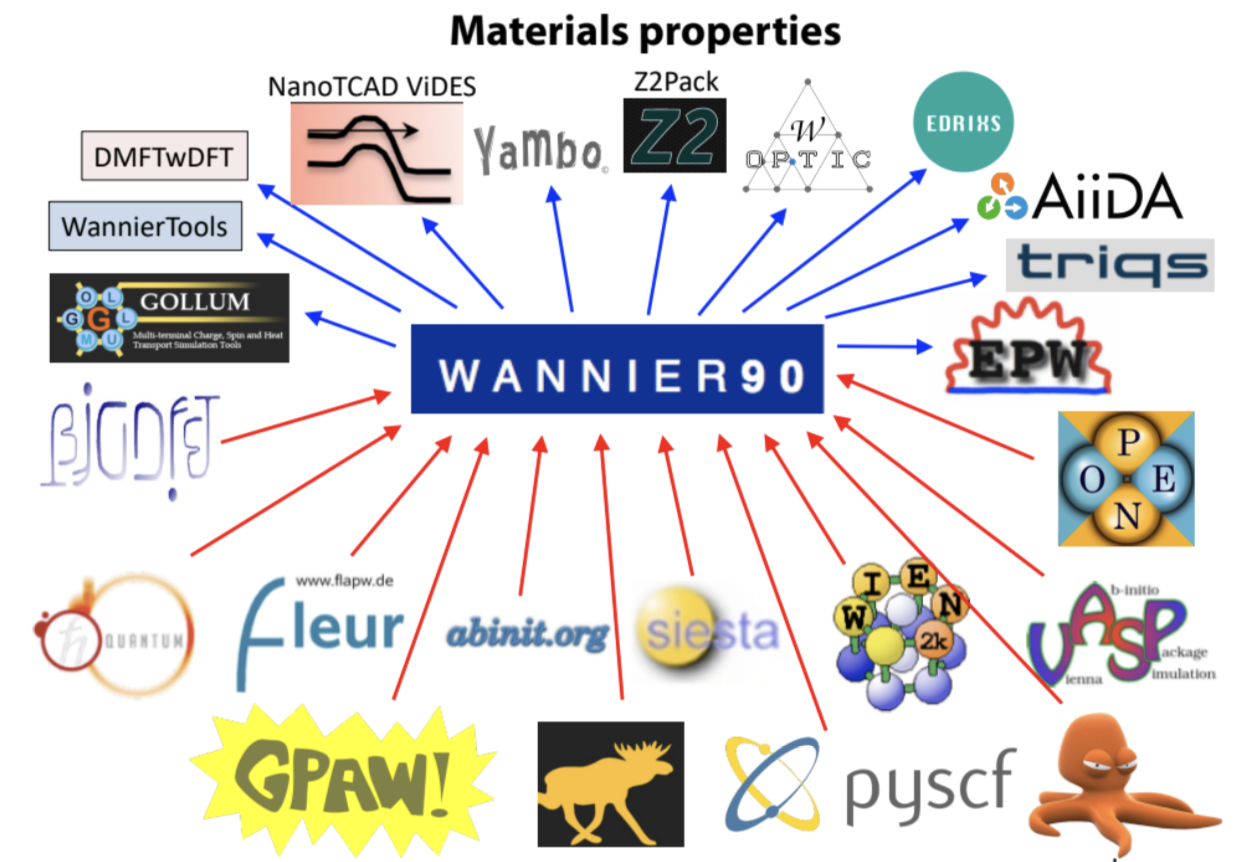
\includegraphics[width=0.5\linewidth]{wannier90.png}
        \caption{Ab initio engines using Wannier90. }
        \item \textit{Computer Physics Communications}, 178(9), 685-699 (2009). Wannier90:\url{http://www.wannier.org/}
    \end{figure}
    \end{frame}
    
    \begin{frame}
    \frametitle{Applications of Wannier Functions}
    \begin{itemize}
        \item Electronic Structure:
        \begin{itemize}
            \item Provides insight into the bonding and electronic properties of materials.
            \item Used for band structure interpolation and analysis.
        \end{itemize}
        \item Polarization and Berryology:
        \begin{itemize}
            \item Electronic polarization, Berry phases, Berry curvature, optical and
            anomalous Hall conductivity,
            orbital magnetization
        \end{itemize}
        \item Topological Insulators:
        \begin{itemize}
            \item Used to study topological invariants, properties and edge states.
        \end{itemize}
        \item Electron-Phonon Interactions:
        \begin{itemize}
            \item Facilitate the calculation of electron-phonon coupling matrices.
        \end{itemize}
        \item Ballistic transport and nanostructures:
        \begin{itemize}
            \item Landauer conductance,
            embedding self-energies,
            large-scale tight binding
        \end{itemize}
        \item Beyond DFT with localized orbitals:
        \begin{itemize}
            \item  Koopmans-Wannier spectral
            functionals, strongly correlated 
            systems with DMFT.
        \end{itemize}
    \end{itemize}
    \end{frame}
    
    \begin{frame}
    \frametitle{Example: Band Structure Interpolation}
    \begin{itemize}
        \item Wannier functions allow for efficient interpolation of band structures.
        \item Essential for calculating accurate electronic properties over the Brillouin zone.
        \item Example: Interpolated band structure of silicon using MLWFs.
    \end{itemize}
    \begin{figure}
        \centering
        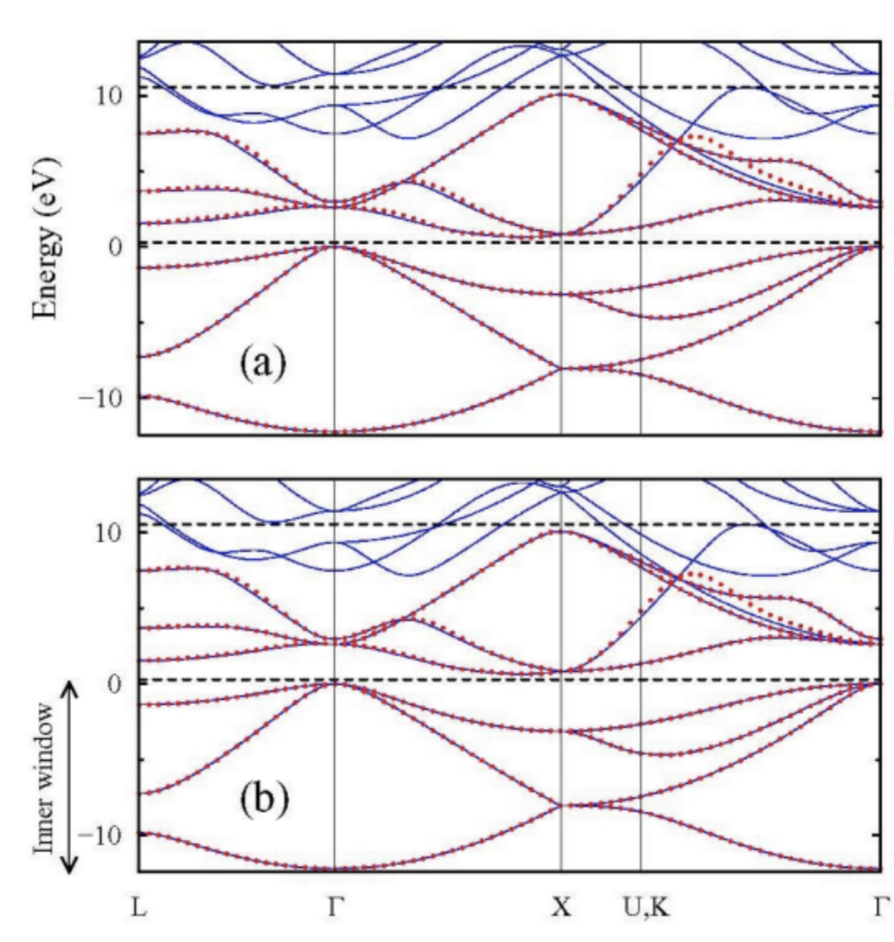
\includegraphics[width=0.3\linewidth]{band_structure.png}
        \caption{Interpolated band structure of silicon using Wannier functions.}
    \end{figure}
    \end{frame}
    
    \iffalse
    \begin{frame}
    \frametitle{Example: Polarization in Ferroelectrics}
    \begin{itemize}
        \item Wannier functions are used to calculate the electronic contribution to polarization in ferroelectric materials.
        \item Example: Polarization change in barium titanate (BaTiO$_3$) during phase transition.
    \end{itemize}
    \begin{figure}
        \centering
        \includegraphics[width=0.8\linewidth]{polarization.png}
        \caption{Polarization change in BaTiO$_3$ calculated using Wannier functions.}
    \end{figure}
    \end{frame}
    \fi
    
    \begin{frame}
    \frametitle{Summary}
    \begin{itemize}
        \item Wannier functions provide a localized representation of electronic states in solids.
        \item They are essential for various applications, including electronic structure, polarization, and topological properties.
        \item Computational tools like Wannier90 facilitate the practical use of Wannier functions.
    \end{itemize}
    \end{frame}



  \coverpage{GW and BSE}
    \section{GW and BSE}
    \begin{frame}
        \frametitle{Introduction to GW Approximation}
        \begin{itemize}
            \item GW is a many-body perturbation theory method used to calculate the electronic structure of materials.
            \item Theoretical framework: the many-body perturbation theory. The Green's function (G) and the screened Coulomb interaction (W).
            \item Beyond DFT method: Provides more accurate quasiparticle energies compared to Density Functional Theory (DFT).
            \item         Moderately correlated systems may be solved numerically
                from first principles using many-body perturbation theory
                (e.g., GW and GW-BSE approaches, and beyond)      
        \end{itemize}
        \end{frame}


        \begin{frame}
        \frametitle{Basic Principles of GW}
        \begin{itemize}
            \item The quasiparticle energy $E_n$ is given by:
            \begin{equation}
            E_n = \epsilon_n + \langle \psi_n | \Sigma(E_n) - V_{xc} | \psi_n \rangle
            \end{equation}
            where $\epsilon_n$ are the Kohn-Sham energies, $\Sigma$ is the self-energy, and $V_{xc}$ is the exchange-correlation potential.
            \item The self-energy $\Sigma$ in the GW approximation is:
            \begin{equation}
            \Sigma(\mathbf{r}, \mathbf{r}'; \omega) = i \int \frac{d\omega'}{2\pi} G(\mathbf{r}, \mathbf{r}'; \omega + \omega') W(\mathbf{r}, \mathbf{r}'; \omega')
            \end{equation}
            where $G$ is the Green's function and $W$ is the screened Coulomb interaction.
        \end{itemize}
        \end{frame}
        
        \begin{frame}
        \frametitle{Computational Steps in GW}
        \begin{itemize}
            \item Start with a DFT calculation to obtain Kohn-Sham eigenvalues and eigenfunctions.
            \item Compute the dielectric function $\epsilon(\mathbf{q}, \omega)$ and the screened Coulomb interaction $W(\mathbf{q}, \omega)$.
            \item Construct the Green's function $G(\mathbf{r}, \mathbf{r}'; \omega)$.
            \item Calculate the self-energy $\Sigma(\mathbf{r}, \mathbf{r}'; \omega)$.
            \item Solve for the quasiparticle energies $E_n$.
        \end{itemize}
        \end{frame}
        
        \begin{frame}
        \frametitle{Introduction to Bethe-Salpeter Equation (BSE)}
        \begin{itemize}
            \item BSE is used to calculate the optical properties of materials by including electron-hole interactions.
            \item Derived from the two-particle Green's function.
            \item Provides accurate excitonic effects and optical spectra.
        \end{itemize}
        \end{frame}
        
        \begin{frame}
        \frametitle{Basic Principles of BSE}
        \begin{itemize}
            \item The BSE describes the correlated motion of an electron-hole pair:
            \begin{equation}
            (\epsilon_c - \epsilon_v) A_{vc} + \sum_{v'c'} K_{vc,v'c'} A_{v'c'} = \Omega A_{vc}
            \end{equation}
            where $\epsilon_c$ and $\epsilon_v$ are the energies of conduction and valence bands, $A_{vc}$ are the exciton amplitudes, $K$ is the electron-hole interaction kernel, and $\Omega$ are the exciton energies.
            \item The kernel $K$ includes the direct Coulomb interaction and the exchange interaction.
        \end{itemize}
        \end{frame}
        
        \begin{frame}
        \frametitle{Computational Steps in BSE}
        \begin{itemize}
            \item Perform a GW calculation to obtain quasiparticle energies and wavefunctions.
            \item Construct the electron-hole interaction kernel $K$.
            \item Solve the BSE to obtain exciton energies $\Omega$ and amplitudes $A_{vc}$.
            \item Calculate the optical absorption spectrum using the exciton amplitudes.
        \end{itemize}
        \end{frame}
        
        \begin{frame}
        \frametitle{Applications of GW and BSE}
        \begin{itemize}
            \item Electronic Structure:
            \begin{itemize}
                \item Provides accurate band gaps and quasiparticle energies.
                \item Essential for studying semiconductors and insulators.
            \end{itemize}
            \item Optical Properties:
            \begin{itemize}
                \item BSE captures excitonic effects in optical spectra.
                \item Important for understanding light absorption and emission in materials.
            \end{itemize}
            \item Materials Design:
            \begin{itemize}
                \item GW and BSE are used to predict and design new materials with desired electronic and optical properties.
            \end{itemize}
        \end{itemize}
        \end{frame}
        
        \begin{frame}
        \frametitle{Example: Band Gap of Silicon}
        \begin{itemize}
            \item GW calculation corrects the underestimated band gap from DFT.
            \item Results show excellent agreement with experimental values.
        \end{itemize}
        \begin{figure}
            \centering
            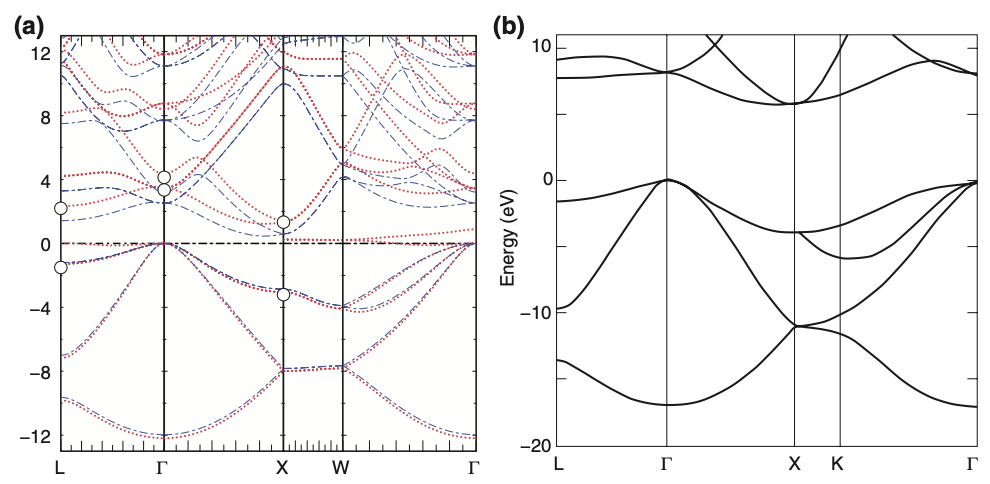
\includegraphics[width=0.7\linewidth]{gw_band_gap.png}
            \caption{Comparison of GW (left) and DFT (right) band gaps for silicon.}
        \end{figure}
        \end{frame}
        
        \begin{frame}
        \frametitle{Example: Optical Spectrum of MoS$_2$}
        \begin{itemize}
            \item BSE captures excitonic peaks in the optical absorption spectrum of monolayer MoS$_2$.
            \item Matches experimental spectra and reveals excitonic binding energies.
        \end{itemize}
        \begin{figure}
            \centering
            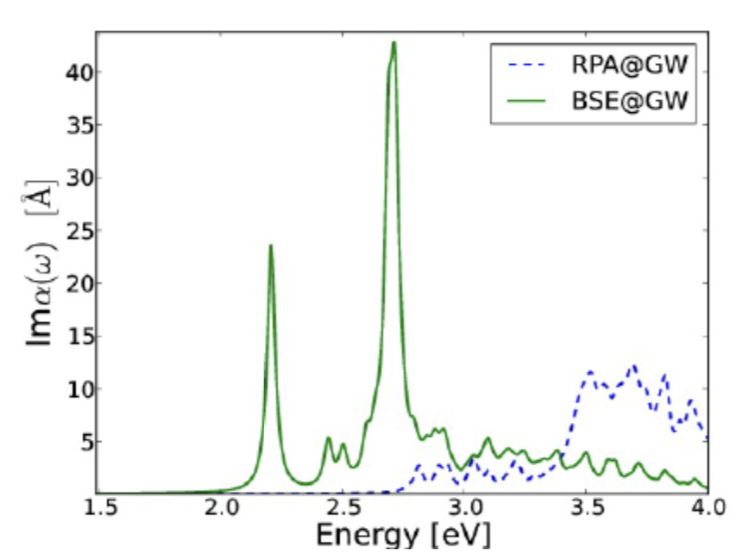
\includegraphics[width=0.4\linewidth]{bse_optical_spectrum.png}
            \caption{  Absorption spectrum of MoS$_2$ calculated with the RPA and BSE using the $G_0W_0$ quasiparticle band structure. (Thygesen PRB 2013)}
        \end{figure}
        \end{frame}

        \begin{frame}
            \frametitle{Example: Optical Spectrum of MoS$_2$}
            \begin{itemize}
                \item BSE captures excitonic peaks in the optical absorption spectrum of monolayer MoS$_2$.
                \item Matches experimental spectra and reveals excitonic binding energies.
            \end{itemize}
            \begin{figure}
                \centering
                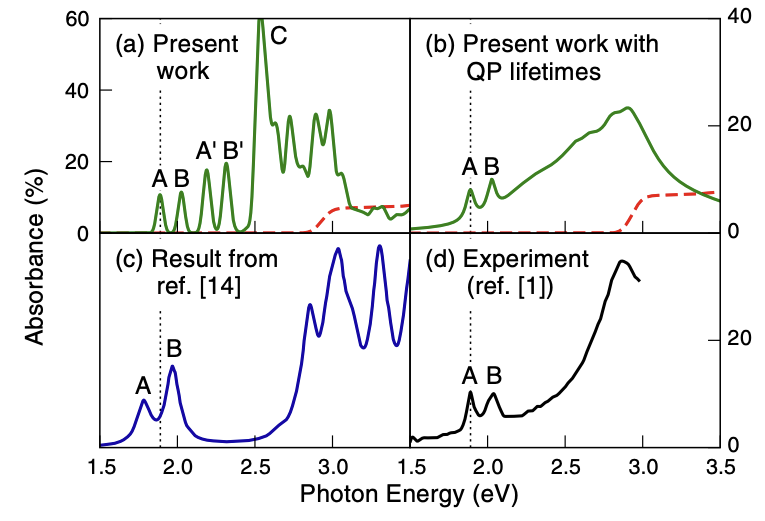
\includegraphics[width=0.4\linewidth]{bse_optical_spectrum2.png}
                \caption{  Absorption spectrum of MoS$_2$ computed using BSE in comparison with experiment. (Diana PRL 2013)}
            \end{figure}
            \end{frame}
        
        \begin{frame}
        \frametitle{Computational Tools for GW and BSE}
        \begin{itemize}
            \item BerkeleyGW: 
            \begin{itemize}
                \item \url{http://www.berkeleygw.org/}
                \item A software package for GW and BSE calculations.
                \item Interfaces with DFT codes like Quantum ESPRESSO and VASP.
            \end{itemize}
            \item Yambo: 
            \begin{itemize}
                \item \url{http://www.yambo-code.org/}
                \item Another package for many-body calculations including GW and BSE.
                \item Capable of handling large systems and complex materials.
            \end{itemize}
        \end{itemize}
        \end{frame}
        
        \begin{frame}
        \frametitle{Summary}
        \begin{itemize}
            \item GW provides accurate quasiparticle energies, improving upon DFT results.
            \item BSE includes electron-hole interactions, essential for accurate optical spectra.
            \item These methods are critical for studying electronic and optical properties of materials.
        \end{itemize}
        \end{frame}
        
        % \begin{frame}
        % \frametitle{References}
        % \begin{itemize}
        %     \item Hedin, L. (1965). New Method for Calculating the One-Particle Green's Function with Application to the Electron-Gas Problem. \textit{Physical Review}, 139(3A), A796.
        %     \item Onida, G., Reining, L., \& Rubio, A. (2002). Electronic excitations: density-functional versus many-body Green's-function approaches. \textit{Reviews of Modern Physics}, 74(2), 601.
        %     \item BerkeleyGW: \url{http://www.berkeleygw.org/}
        %     \item Yambo: \url{http://www.yambo-code.org/}
        % \end{itemize}
        % \end{frame}
    

    


% DFPT
\section{DFPT}
\coverpage{DFPT}
\begin{frame}
    \frametitle{Introduction to DFPT}
    \begin{itemize}
        \item DFPT is an extension of Density Functional Theory (DFT) for studying the response of a system to small perturbations.
        \item It allows for the calculation of phonons, dielectric properties, and electron-phonon interactions.
        \item Developed to overcome the limitations of finite-difference methods in calculating response functions.
    \end{itemize}
    \end{frame}
    
    \begin{frame}
    \frametitle{Basic Principles}
    \begin{itemize}
        \item DFT provides the ground-state properties of a many-electron system using the electron density $\rho(\mathbf{r})$.
        \item DFPT extends DFT to linear response theory, allowing the calculation of changes in $\rho(\mathbf{r})$ due to a perturbation.
        \item The perturbation can be an external electric field, atomic displacement, etc.
    \end{itemize}
    \end{frame}
    
    \begin{frame}
    \frametitle{Linear Response Theory}
    \begin{itemize}
        \item The response of the electron density $\rho(\mathbf{r})$ to a perturbation $V_{\text{ext}}(\mathbf{r})$ can be expressed as:
        \begin{equation}
        \delta \rho(\mathbf{r}) = \int \chi(\mathbf{r}, \mathbf{r}') \delta V_{\text{ext}}(\mathbf{r}') d\mathbf{r}'
        \end{equation}
        where $\chi(\mathbf{r}, \mathbf{r}')$ is the density-density response function.
        \item DFPT calculates $\chi(\mathbf{r}, \mathbf{r}')$ using perturbation theory within the DFT framework.
    \end{itemize}
    \end{frame}
    
    \begin{frame}
    \frametitle{Key Equations in DFPT}
    \begin{itemize}
        \item The self-consistent field (SCF) equations in DFT are modified to include the perturbation:
        \begin{equation}
        \left( -\frac{\hbar^2}{2m} \nabla^2 + V_{\text{eff}}[\rho_0](\mathbf{r}) + \delta V_{\text{eff}}[\delta \rho](\mathbf{r}) \right) \psi_i(\mathbf{r}) = \epsilon_i \psi_i(\mathbf{r})
        \end{equation}
        \item Here, $V_{\text{eff}}$ is the effective potential, and $\delta V_{\text{eff}}$ is its variation due to the perturbation.
    \end{itemize}
    \end{frame}
    
    \begin{frame}
    \frametitle{Applications of DFPT}
    \begin{itemize}
        \item Phonon Calculations:
        \begin{itemize}
            \item Determines the vibrational modes and frequencies of a crystal.
            \item Used to study thermal properties and stability of materials.
        \end{itemize}
        \item Dielectric Properties:
        \begin{itemize}
            \item Calculates the dielectric constant and piezoelectric tensors.
            \item Important for understanding material responses to electric fields.
        \end{itemize}
        \item Electron-Phonon Interactions:
        \begin{itemize}
            \item Computes electron-phonon coupling constants.
            \item Essential for studying superconductivity and electrical conductivity.
        \end{itemize}

        Baroni, S., de Gironcoli, S., Dal Corso, A., \& Giannozzi, P. (2001). Phonons and related crystal properties from density-functional perturbation theory. \textit{Reviews of Modern Physics}, 73(2), 515.

    \end{itemize}
    \end{frame}
    
    % \begin{frame}
    % \frametitle{Example: Phonon Dispersion in Silicon}
    % \begin{itemize}
    %     \item Phonon dispersion relations describe how phonon frequencies vary with wavevector.
    %     \item DFPT is used to calculate the phonon dispersion of silicon, a key material in electronics.
    %     \item Results match well with experimental data, validating the accuracy of DFPT.
    % \end{itemize}
    % \begin{figure}
    %     \centering
    %     \includegraphics[width=0.8\linewidth]{phonon_dispersion_si.png}
    %     \caption{Phonon dispersion of silicon calculated using DFPT.}
    % \end{figure}
    % \end{frame}
    
    % \begin{frame}
    % \frametitle{Computational Tools for DFPT}
    % \begin{itemize}
    %     \item Quantum ESPRESSO:
    %     \begin{itemize}
    %         \item Open-source software for DFT and DFPT calculations.
    %         \item Provides modules for phonon calculations, dielectric properties, and electron-phonon interactions.
    %     \end{itemize}
    %     \item ABINIT:
    %     \begin{itemize}
    %         \item Another open-source package for DFT and DFPT.
    %         \item Used for similar calculations as Quantum ESPRESSO.
    %     \end{itemize}
    % \end{itemize}
    % \end{frame}
    
    \begin{frame}
    \frametitle{Summary}
    \begin{itemize}
        \item DFPT extends DFT to study the response of systems to small perturbations.
        \item It is crucial for calculating phonons, dielectric properties, and electron-phonon interactions.
        \item Widely used in material science to predict and understand physical properties.
    \end{itemize}
    \end{frame}
    
    % \begin{frame}
    % \frametitle{References}
    % \begin{itemize}
    %     \item Baroni, S., de Gironcoli, S., Dal Corso, A., \& Giannozzi, P. (2001). Phonons and related crystal properties from density-functional perturbation theory. \textit{Reviews of Modern Physics}, 73(2), 515.
    %     \item Quantum ESPRESSO: \url{http://www.quantum-espresso.org/}
    %     \item ABINIT: \url{https://www.abinit.org/}
    % \end{itemize}
    % \end{frame}
 

    \begin{frame}
        \frametitle{Conclusion}
        \begin{itemize}
            \item Comprehensive coverage of electron-phonon physics and computational methods
            \item Balance of theoretical lectures and practical tutorials
            \item Importance of hands-on experience with state-of-the-art tools
            % \item Networking and collaborative opportunities
        \end{itemize}
        \end{frame}

        

    \coverpage{Supplimentary and Misc.}
    \section*{Misc.}

    \begin{frame}
        \frametitle{CECAM Flagship Workshop}
        \begin{itemize}
        \item      Frontiers in many-body excited-state dynamics from first principles
        \end{itemize}
    \begin{figure}
        \centering
        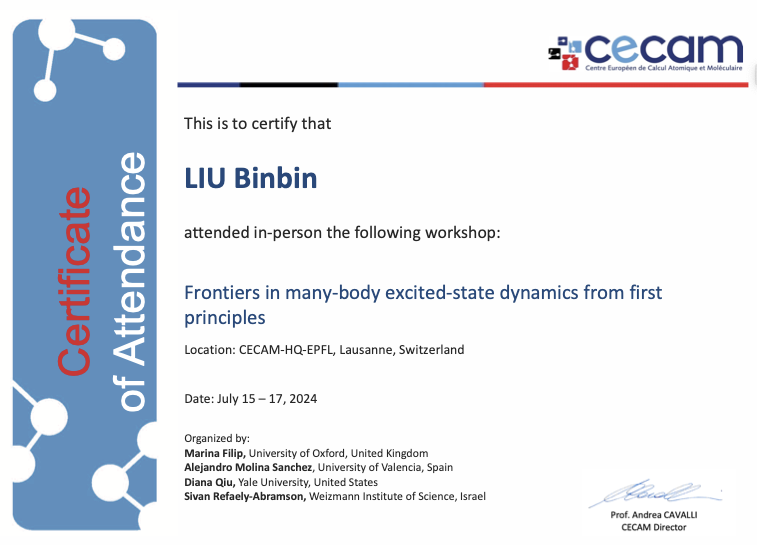
\includegraphics[width=0.6\linewidth]{cecam.png}
        % \caption{            }
    \end{figure}
    \end{frame}

        \begin{frame}
            \frametitle{Wannierize Exitonic Bands (from the CECAM workshop) }
            \begin{itemize}
                \item   Maximally-Localized Exciton Wannier Functions (Haber, Qiu, da Jornada, Neaton, Phys. Rev. B 108, 125118 (2023)).
                \item A new representation of excitons enabling tight-binding models, geometric phases, interpolation, and physical interpretation
                \item Interface with Wannier90 different workflows. (Special treatment to the non-analytic term.)
                \item → MLXWFs can be a good localized basis for exciton-polaron physics. (Dai, Lian, Lafuente-Bartolome, Giustino, Phys. Rev. B 109, 045202 (2024))
                \begin{figure}
                    \centering
                    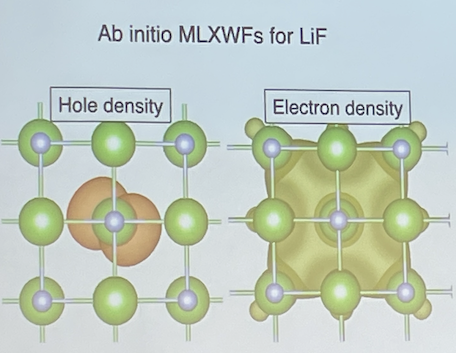
\includegraphics[width=0.3\linewidth]{exitonwannier.png}
                    \caption{Ab initio MLXWFs for LiF(From: Neaton's group at Berkeley.)            }
                \end{figure}
            \end{itemize}
            \end{frame}

            \begin{frame}
                \frametitle{Properties of Weyl semimetal (may be interesting)}
                \begin{itemize}
                   \item Thermoelectric: Practical efforts to achieve low-temperature thermoelectrics using nodal loop semimetals may therefore find it fruitful to identify materials with a nearly flat nodal line. (PRXEnergy.3.023007)   
                   \item Exitonic effects in Weyl semimetals.
                   \item Exiton in Weyl phonons: no research paper on this so far!
                \end{itemize}
            \end{frame}

            \begin{frame}
                \frametitle{Applications of Direct Band Gap Semiconductor}
                \begin{itemize}
    Optoelectronic devices: Direct band gap materials, with their high radiative recombination rates and strong absorption of light, are widely used in the development of lasers, LEDs, and photodetectors. These devices rely on efficient light emission and absorption for their operation.
    Solar cells: Direct band gap materials are also utilized in solar cells, where their high absorption coefficient enables efficient conversion of sunlight into electricity.
            \end{itemize}
            \begin{figure}
                \centering
                
\includegraphics[width=0.4\linewidth]{solarcity.png}
                \caption{Solar city (Tesla)            }
            \end{figure}
            \end{frame}
  
            \begin{frame}
                    \frametitle{Literature Reviews on GW and BSE}
                    \begin{itemize}
                        \item The GW method, F Aryasetiawan and O Gunnarsson, 1998 Rep. Prog. Phys. 61 237 
                        \item Electronic excitations: density-functional versus many-body Green’s-function approaches, REVIEWS OF MODERN PHYSICS, VOLUME 74, APRIL 2002 
                        \item Calculating excitons, plasmons, and quasiparticles in 2D materials and van der Waals heterostructures, Kristian Sommer Thygesen
                        \item The GW approximation: content, successes and limitations, Lucia Reining
                        \item The GW Compendium: A Practical Guide to Theoretical Photoemission Spectroscopy
                        Dorothea Golze* Marc Dvorak and Patrick Rinke %https://www.frontiersin.org/journals/chemistry/articles/10.3389/fchem.2019.00377/full
                    \end{itemize}
                    \end{frame}
            
                
\end{document}

